\documentclass[a5paper,10pt]{article}
 
\usepackage{extsizes}
\usepackage{cmap}
\usepackage[T2A]{fontenc}
\usepackage[utf8x]{inputenc}
% \usepackage[russian]{babel}
\usepackage[english, russian]{babel}
% \usepackage{newtx}
% \usepackage{cyrtimes}
\usepackage{misccorr}

%%%%%%%%%%%%%%%%%%%%%%%%%%%%%%%%%%%%%%%%%%%%%%%%%%%%%%%%%%%%%%%%%%%%%%%%%%%%%%%%%%  
\usepackage{graphicx} % для вставки картинок
\graphicspath{{img/}}
\usepackage{amssymb,amsfonts,amsmath,amsthm} % математические дополнения от АМС

% \usepackage{fontspec}
% \usepackage{unicode-math}

\usepackage{indentfirst} % отделять первую строку раздела абзацным отступом тоже
\usepackage[usenames,dvipsnames]{color} % названия цветов
\usepackage{makecell}
\usepackage{multirow} % улучшенное форматирование таблиц
\usepackage{ulem} % подчеркивания
\linespread{1.3} % полуторный интервал
% \renewcommand{\rmdefault}{ftm} % Times New Roman (не работает)
\frenchspacing
\usepackage{geometry}
\geometry{left=1cm,right=1cm,top=2cm,bottom=1cm,bindingoffset=0cm}
\usepackage{titlesec}
\usepackage{float}
% \definecolor{black}{rgb}{0,0,0}
% \usepackage[colorlinks, unicode, pagecolor=black]{hyperref}
% \usepackage[unicode]{hyperref} %ссылки
\usepackage{fancyhdr} %загрузим пакет
\pagestyle{fancy} %применим колонтитул
\fancyhead{} %очистим хидер на всякий случай
\fancyhead[LE,RO]{Сарафанов Ф.Г.} %номер страницы слева сверху на четных и справа на нечетных
\fancyhead[CO, CE]{Механика}
\fancyhead[LO,RE]{№269 -- Яковлев И.А.} 
\fancyfoot{} %футер будет пустой
% \fancyfoot[CO,CE]{\thepage}
\renewcommand{\labelenumii}{\theenumii)}
\newcommand{\ddt}{$\ \pm\ 0.2\ \text{с}$}
\newcommand{\ddtv}{$\ \pm\ 0.8\ \text{с}$}
\newcommand{\ddh}{$\ \pm\ 0.1\ \text{см}$}

\usepackage{amsthm}
\newtheorem{define}{Определение}
\newtheorem{theorem}{Теорема}
\newtheorem{problem}{Задача}

\begin{document}
% \pagestyle{empty}
% \thispagestyle{empty}
\begin{figure}[H]
	\centering
	\vspace{-1em}
	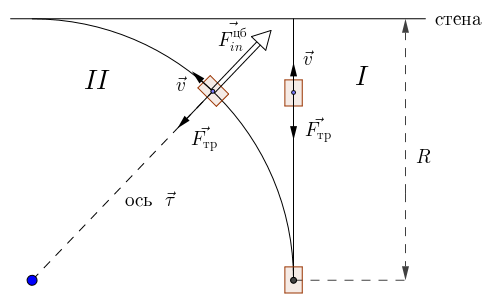
\includegraphics[width=0.96\textwidth]{269-2.png}
	% \caption{Caption }
	% \label{fig:figure1}
\end{figure}
\textbf{Случай $I$.} Рассмотрим движение с торможением без поворота. В проекции на перпендикуляр к стене:

$v=v_0+at$, по 2 закону Ньютона $ma=-F_\text{тр}$, $a=-g\mu$. Тогда можем найти время до остановки $t^*$:
\vspace{-1em}
$$v_\text{ост}=0=v_0-g\mu{}t^* \Longrightarrow t^*=\frac{v_0}{g\mu}$$
% \vspace{-1em}
Тогда из уравнения движения находим пройденное до остановки расстояние $R$:
% \vspace{-0.5em}
$$R=v_0\cdot{t^*}+\frac{a{t^*}^2}{2}=\frac{v_0^2}{g\mu}-\frac{g\mu{}v_0^2}{2(g\mu)^2}=\frac{v_0^2}{2g\mu}$$
% \vspace{-1em}

\textbf{Случай $II$.} Перейдем в НИСО, связанную с автомобилем. НИСО тогда вращается с $\omega=v/r$, а 2 зн. Ньютона запишется как $m\vec{a}'=0=\vec{F}_\text{тр}+\vec{F_{in}^\text{цб}}$. В проекции на $\tau$: $m\omega^2R=g\mu$, Отсюда $$R=\frac{v^2}{g\mu}$$.
\\

\textbf{Вывод.} Торможение без поворота позволит остановится вдвое раньше, чем поворот без торможения и заноса.

\end{document}

